 \subsubsection{Passive 2-Tore} \label{subsubsec:2tore}
  
Passive 2-Tore sind Netzwerke mit 2 Klemmenpaaren, die in jedem Betriebszustand Leistung verbrauchen. Ein Klemmenpaar wird auch als Tor bezeichnet. Dabei wird ein Tor als Eingang für ein elektrisches Signal verwendet. Folglich wird am anderen Tor das Ausgangssignal abgegriffen. Ein Netzwerk, das intern nur aus beliebigen R-(ohmischer Widerstand), L-(Induktivität), C-(Kapazität) und M-(Gegeninduktivität) Komponenten aufgebaut ist, ist immer ein passives Netzwerk. Ein solches 2-Tor ist in der Abbildung \ref{fig:2tor} dargestellt.

\begin{figure}[H]
	\centering
	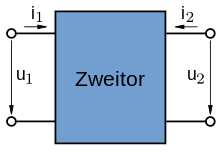
\includegraphics[width=8cm]{2Tor.png}
	\caption{Zweitor (2-Tor) \textcolor{red}{\textbf{TODO:Quelle Bild}} }
	\label{fig:2tor}
\end{figure}

Ein solches Netzwerk ist zusätzlich noch reziprok. Reziproke Netzwerke haben die Eigenschaft, dass es egal ist, in welche Richtung sie betrieben werden, solange der Innenwiderstand der Quelle gleich gross wie die Lastimpedanz ist. Anhand vom folgenden Beispiel (Abbildung: \ref{fig:reziprozitat}) wird dies veranschaulicht. Die Leistung im Verbraucher ist in beiden Betriebszuständen dieselbe. Mit dieser Eigenschaft können in der  Praxis die Berechnungen sehr vereinfacht werden. \textcolor{red}{\textbf{TODO:Quelle Inhalt}}

\begin{figure}[H]
	\centering
	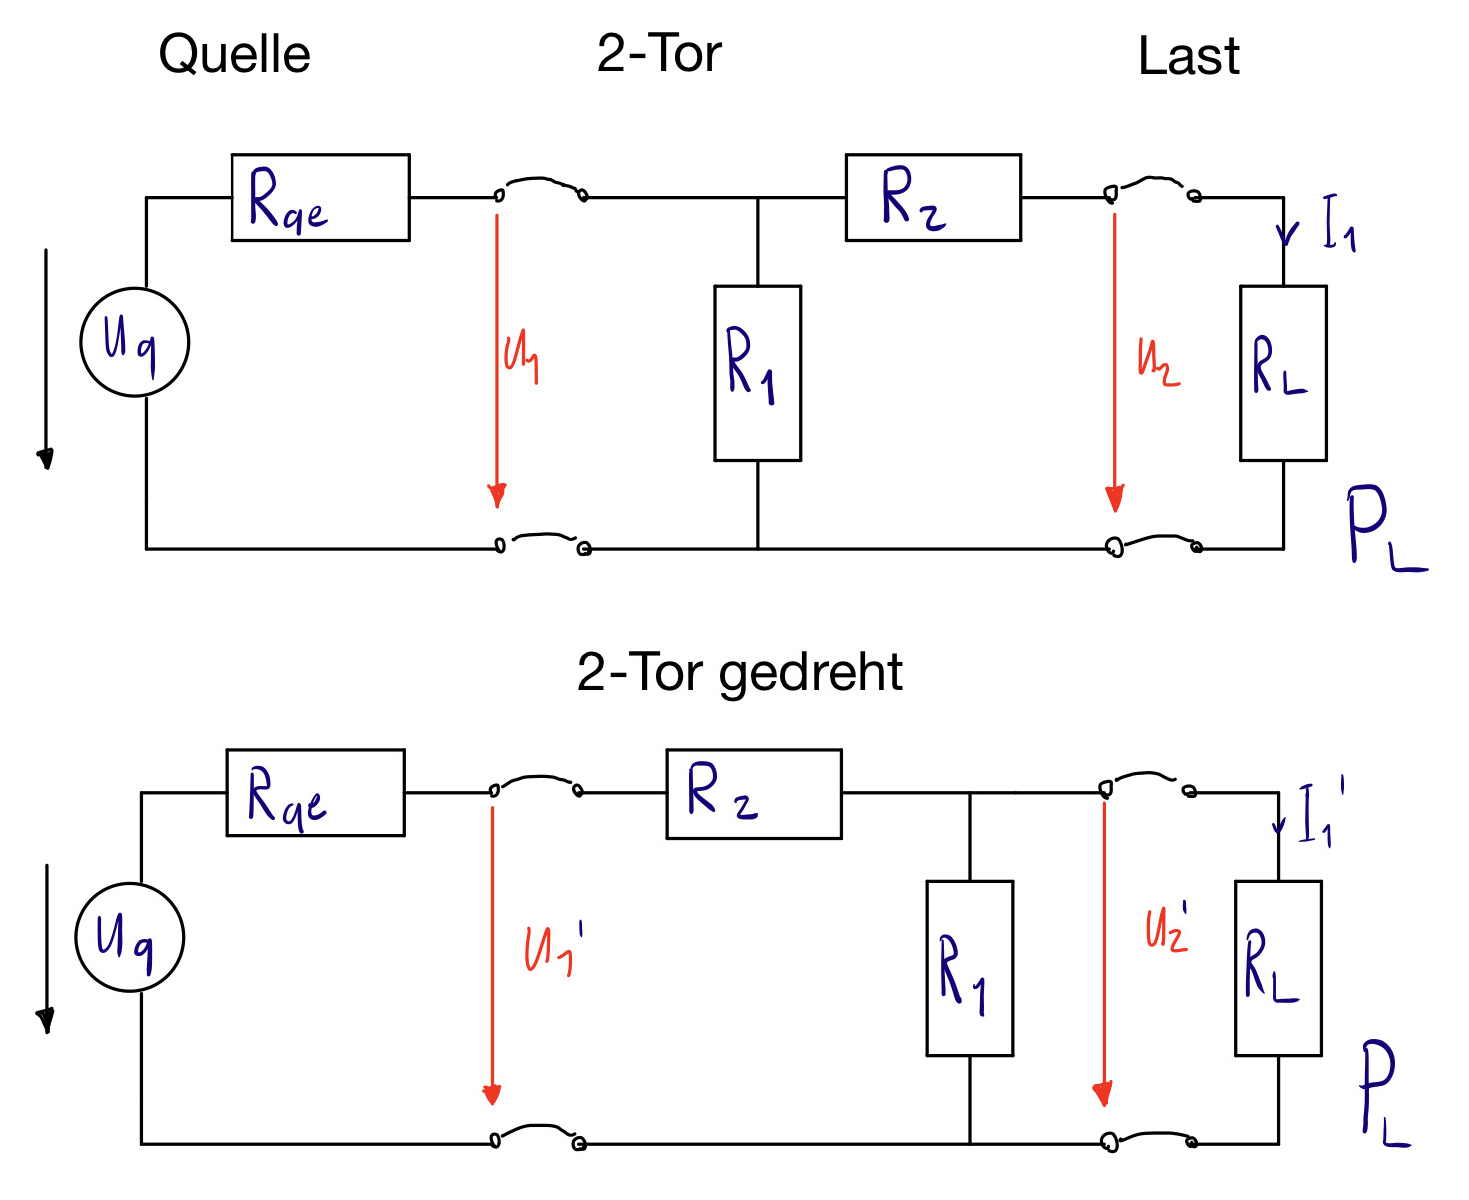
\includegraphics[width=10cm]{bsp_reziprok.png}
	\caption{Beispiel Reziprozitat}
	\label{fig:reziprozitat}
\end{figure}


Als Beispiel sind R$_qe$ und R$_L$ jeweils 50 Ohm, R$_1$ 150 Ohm und R$_2$ 20 Ohm. Die Quelle hat eine Spannung von 100V.

In beiden Netzwerken berechnen wir aus der Quelle und dem 2-Tor den Ersatzwiderstand  R$_q_1$ und R$_q_2$.


\begin{equation}\label{equ:rqe1}
			R_{q1} = \frac{1}{\frac{1}{R_Q}+\frac{1}{R_1}} +R_2 =  57.5 \Omega 
		\end{equation}

\begin{equation}\label{equ:rqe1}
			R_{q2} = \frac{1}{\frac{1}{R_Q+R_2}+\frac{1}{R_1}} =  47.73 \Omega 
		\end{equation}
	
\textcolor{red}{\textbf{TODO:Berechnungen fertig machen und aufzeigen warum Ib=Ib und Ub und Ub}}	

\begin{figure}[H]
	\centering
	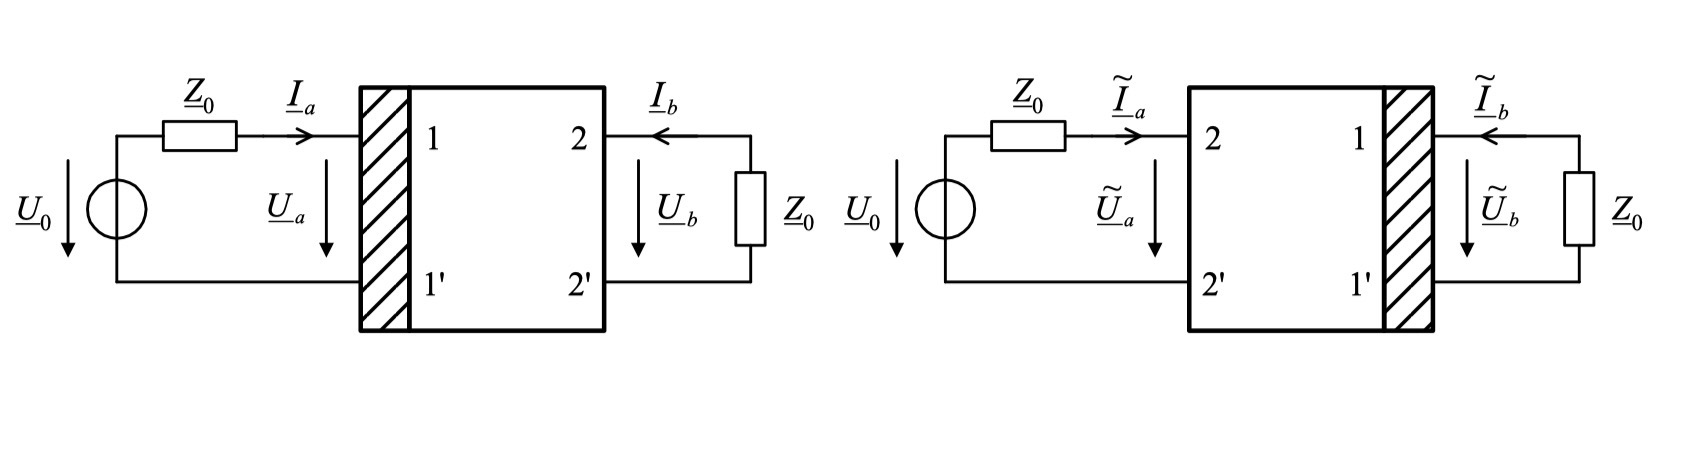
\includegraphics[width=12cm]{reziprozitat.jpg}
	\label{fig:reziprozitat}
\end{figure}

Im dargestellten Netzwerk gilt somit

\begin{equation}\label{equ:verticImpedance}
			\underline{I}_b =  \underline{\tilde{I}}_b
		\end{equation}
		
sowie 		
		
\begin{equation}\label{equ:verticImpedance}
			\underline{U}_b =  \underline{\widetilde{U}}_b
		\end{equation}

\newpage


